% Standalone comparison document: old (originally-published) vs revised
% numbers for the TMLR paper. Each table cell renders unchanged values
% as-is and changed values as \chg{old}{new} -- a small, struck-through
% old in grey followed by the new value -- so a glance shows what shifted.
%
% Generated by:
%   results/benchmark_table_comparison.py  -> tables/benchmark_{nacl,cscl,cu2o}_comparison.tex
%   results/biodimers_comparison.py        -> tables/biodimers_comparison.tex
%
% Compile standalone (pdflatex comparison.tex) or \input into main.tex.

\documentclass[11pt]{article}

\usepackage[a4paper,margin=2cm]{geometry}
\usepackage{graphicx}
\usepackage{booktabs}
\usepackage{makecell}
\usepackage[separate-uncertainty=true,exponent-product=\cdot]{siunitx}
\usepackage{chemformula}
\usepackage{xcolor}
\usepackage[normalem]{ulem}
\usepackage{caption}
\usepackage{hyperref}
\usepackage[capitalise]{cleveref}
\captionsetup[table]{skip=6pt}

% Force-vector shorthand mirrors main.tex.
\newcommand{\F}{\mathbf{F}}

% \chg{old}{new}: small struck-through old in grey, then new value.
% Used by every comparison table cell that actually shifted.
\newcommand{\chg}[2]{{\scriptsize\color{black!45}\sout{#1}}\,#2}

\title{TMLR paper: old vs revised data\\
\large \textit{Learning Long-Range Representations with Equivariant Messages}}
\author{}
\date{}

\begin{document}
\maketitle

\noindent
Each table cell shows either the unchanged value or
\chg{\textit{old}}{\textit{new}} when the number shifted. Old values are
the originally-published numbers; new values are
the revised numbers.

\section*{Biodimers totals}

Per-class indexing bug in the LOREM evaluation driver. Totals over the
full biodimers test set are essentially unchanged (within 3-decimal
rounding) for every variant except \textsc{Lorem} LR $l=0$, which
turned out to be the variant whose pre-fix totals were genuinely
different. The starred ($\dagger$) ablation seeds were unaffected. Per-class results, \cref{fig:bio-comparison}, changed significantly.

\begin{table}[ht]
  \centering
  \caption{Biodimers test-set totals across LOREM variants.}
  \begin{tabular}{l | r r r r}
\toprule
  \multicolumn{1}{c}{} & \multicolumn{4}{c}{Biodimers (test set, total)} \\ 
                   Variant  &           $E$ RMSE (meV/at)  &            $E$ MAE (meV/at)  &           $\F$ RMSE (meV/Å)  &            $\F$ MAE (meV/Å) \\ 
\midrule
            \textsc{Lorem}  &                 \num{0.222}  &                 \num{0.155}  &                 \num{1.646}  &                 \num{1.023} \\ 
\textsc{Lorem}$^{\dagger}$  &                 \num{0.370}  &                 \num{0.322}  &                 \num{1.985}  &                 \num{1.110} \\ 
   \textsc{Lorem} LR $l=0$  &                 \num{0.302}  &                 \num{0.268}  &                 \num{1.677}  &                 \num{1.010} \\ 
\textsc{Lorem} LR $l=0^{\dagger}$  &                 \num{0.431}  &                 \num{0.255}  &                 \num{1.838}  &                 \num{1.124} \\ 
   \textsc{Lorem} LR $l=1$  &                 \num{0.329}  &                 \num{0.203}  &                 \num{1.725}  &                 \num{0.981} \\ 
\textsc{Lorem} LR $l=1^{\dagger}$  &                 \num{0.329}  &                 \num{0.302}  &                 \num{1.698}  &                 \num{1.043} \\ 
      \textsc{Lorem} no LR  &                 \num{8.259}  &                 \num{3.784}  &                \num{16.452}  &                 \num{5.468} \\ 
\textsc{Lorem} no LR$^{\dagger}$  &                 \num{8.978}  &                 \num{3.934}  &                \num{16.381}  &                 \num{5.588} \\ 
\bottomrule
\end{tabular}

\end{table}

The per-class breakdown is where the bug actually shows; Fig.~\ref{fig:bio-comparison} reproduces the main-text MAE plot with an extra faded \textsc{Lorem} bar carrying the originally-published per-class numbers.

\begin{figure}[ht]
  \centering
  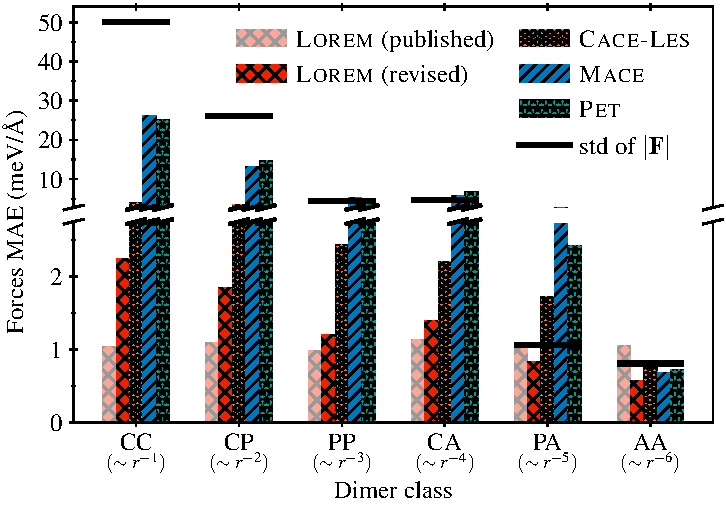
\includegraphics[width=0.95\linewidth]{figures/biodimers_comparison}
  \caption{Per-class force MAE on biodimers (the main-text figure). The faded \textsc{Lorem} bar in each class group is the originally-published number; the bold \textsc{Lorem} bar is the corrected value. \textsc{Cace-Les}, \textsc{Mace}, and \textsc{Pet} are unchanged. Source: \texttt{results/biodimers\_figure\_comparison.py}.}
  \label{fig:bio-comparison}
\end{figure}

\clearpage


\section*{Benchmark timings (Appendix E)}

The Ewald-vs-PME timing tables shifted because the original benchmark
ran Ewald and PME at mismatched accuracy. The revised \emph{light}
regime fixes the PME accuracy target while letting Ewald reach larger
$N$ thanks to the smaller $k$-grid. \texttt{nolr} was also re-run so the LR-fraction breakdown is apples-to-apples.

\begin{figure}[ht]
  \centering
  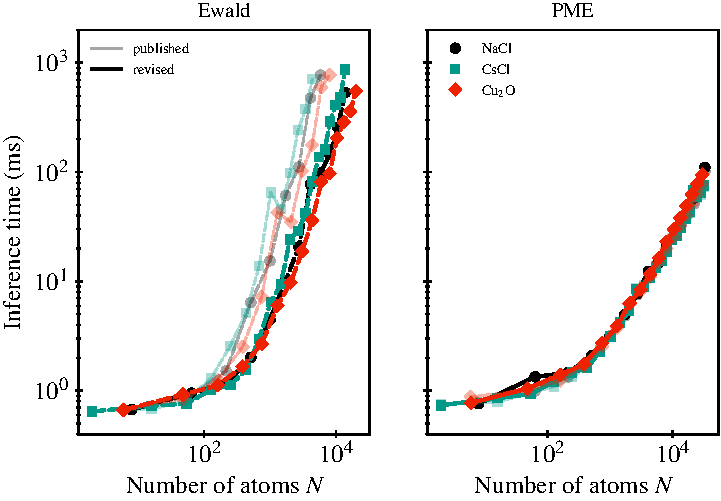
\includegraphics[width=0.95\linewidth]{figures/benchmark_comparison_light}
  \caption{Light-regime benchmark: original (faded) vs revised (bold)
    timings for all three crystals. Ewald dashed, PME solid. Source:
    \texttt{results/benchmark\_comparison\_figure.py}.}
\end{figure}

\begin{table}[ht]
  \centering
  \caption{NaCl: Ewald vs PME, LR breakdown.}
  \begin{tabular}{r | r r r | r r r}
\toprule
  \multicolumn{1}{c}{} & \multicolumn{3}{c}{Ewald} & \multicolumn{3}{c}{PME} \\ 
                   $N$  &              SR+LR (ms)  &                 LR (ms)  &                 LR (\%)  &              SR+LR (ms)  &                 LR (ms)  &                 LR (\%) \\ 
\midrule
                     8  &               \num{0.7}  &  \chg{\num{0.2}}{\num{0.3}}  &  \chg{\num{32.4}}{\num{40.7}}  &               \num{0.8}  &  \chg{\num{0.3}}{\num{0.4}}  &  \chg{\num{41.9}}{\num{47.6}} \\ 
                    64  &  \chg{\num{0.9}}{\num{1.0}}  &               \num{0.4}  &  \chg{\num{45.4}}{\num{43.1}}  &  \chg{\num{1.0}}{\num{1.3}}  &  \chg{\num{0.5}}{\num{0.8}}  &  \chg{\num{50.0}}{\num{59.6}} \\ 
%                    216  &  \chg{\num{1.5}}{\num{1.2}}  &  \chg{\num{0.8}}{\num{0.4}}  &  \chg{\num{52.1}}{\num{32.0}}  &  \chg{\num{1.3}}{\num{1.5}}  &  \chg{\num{0.6}}{\num{0.7}}  &  \chg{\num{45.6}}{\num{46.3}} \\ 
                   512  &  \chg{\num{6.4}}{\num{2.0}}  &  \chg{\num{5.3}}{\num{0.9}}  &  \chg{\num{82.6}}{\num{42.9}}  &               \num{2.1}  &  \chg{\num{1.0}}{\num{0.9}}  &  \chg{\num{46.0}}{\num{44.6}} \\ 
%                   1000  &  \chg{\num{15.4}}{\num{4.5}}  &  \chg{\num{13.6}}{\num{2.6}}  &  \chg{\num{88.4}}{\num{57.3}}  &  \chg{\num{3.2}}{\num{3.1}}  &  \chg{\num{1.4}}{\num{1.2}}  &  \chg{\num{43.3}}{\num{39.2}} \\ 
                  1728  &  \chg{\num{61.2}}{\num{10.2}}  &  \chg{\num{58.4}}{\num{7.3}}  &  \chg{\num{95.5}}{\num{71.3}}  &  \chg{\num{4.8}}{\num{5.0}}  &  \chg{\num{2.1}}{\num{2.0}}  &  \chg{\num{42.6}}{\num{40.8}} \\ 
%                   2744  &  \chg{\num{111.7}}{\num{20.7}}  &  \chg{\num{107.6}}{\num{16.2}}  &  \chg{\num{96.3}}{\num{78.5}}  &  \chg{\num{7.6}}{\num{7.7}}  &  \chg{\num{3.4}}{\num{3.3}}  &  \chg{\num{45.1}}{\num{42.7}} \\ 
                  4096  &  \chg{\num{475.8}}{\num{77.5}}  &  \chg{\num{469.8}}{\num{71.0}}  &  \chg{\num{98.7}}{\num{91.6}}  &  \chg{\num{12.1}}{\num{12.3}}  &  \chg{\num{6.1}}{\num{5.8}}  &  \chg{\num{50.5}}{\num{47.2}} \\ 
%                   5832  &  \chg{\num{773.3}}{\num{97.9}}  &  \chg{\num{765.0}}{\num{88.8}}  &  \chg{\num{98.9}}{\num{90.8}}  &  \chg{\num{14.5}}{\num{14.8}}  &  \chg{\num{6.2}}{\num{5.7}}  &  \chg{\num{42.4}}{\num{38.8}} \\ 
                  8000  &   \chg{--}{\num{145.1}}  &   \chg{--}{\num{132.3}}  &    \chg{--}{\num{91.2}}  &  \chg{\num{20.2}}{\num{21.1}}  &  \chg{\num{8.9}}{\num{8.3}}  &  \chg{\num{43.8}}{\num{39.3}} \\ 
%                  10648  &   \chg{--}{\num{257.4}}  &   \chg{--}{\num{239.3}}  &    \chg{--}{\num{93.0}}  &  \chg{\num{26.1}}{\num{28.8}}  &  \chg{\num{11.2}}{\num{10.7}}  &  \chg{\num{42.9}}{\num{37.3}} \\ 
%                  13824  &   \chg{--}{\num{534.4}}  &   \chg{--}{\num{510.4}}  &    \chg{--}{\num{95.5}}  &  \chg{\num{33.5}}{\num{37.4}}  &  \chg{\num{14.1}}{\num{13.4}}  &  \chg{\num{42.0}}{\num{35.8}} \\ 
                 17576  &                      --  &                      --  &                      --  &  \chg{\num{41.5}}{\num{46.3}}  &  \chg{\num{16.9}}{\num{15.7}}  &  \chg{\num{40.7}}{\num{33.9}} \\ 
%                  21952  &                      --  &                      --  &                      --  &  \chg{\num{51.3}}{\num{58.0}}  &  \chg{\num{20.1}}{\num{18.7}}  &  \chg{\num{39.1}}{\num{32.3}} \\ 
%                  27000  &                      --  &                      --  &                      --  &  \chg{\num{65.8}}{\num{75.8}}  &  \chg{\num{26.8}}{\num{25.4}}  &  \chg{\num{40.7}}{\num{33.5}} \\ 
                 32768  &                      --  &                      --  &                      --  &  \chg{\num{101.2}}{\num{110.6}}  &  \chg{\num{51.6}}{\num{46.9}}  &  \chg{\num{51.0}}{\num{42.4}} \\ 
%                  39304  &                      --  &                      --  &                      --  &   \chg{--}{\num{113.7}}  &    \chg{--}{\num{35.7}}  &    \chg{--}{\num{31.4}} \\ 
%                  46656  &                      --  &                      --  &                      --  &   \chg{--}{\num{138.0}}  &    \chg{--}{\num{44.3}}  &    \chg{--}{\num{32.1}} \\ 
%                  54872  &                      --  &                      --  &                      --  &   \chg{--}{\num{163.0}}  &    \chg{--}{\num{51.5}}  &    \chg{--}{\num{31.6}} \\ 
%                  64000  &                      --  &                      --  &                      --  &   \chg{--}{\num{218.1}}  &    \chg{--}{\num{88.1}}  &    \chg{--}{\num{40.4}} \\ 
%                  74088  &                      --  &                      --  &                      --  &   \chg{--}{\num{217.8}}  &    \chg{--}{\num{66.2}}  &    \chg{--}{\num{30.4}} \\ 
%                  85184  &                      --  &                      --  &                      --  &   \chg{--}{\num{256.9}}  &    \chg{--}{\num{82.4}}  &    \chg{--}{\num{32.1}} \\ 
\bottomrule
\end{tabular}

\end{table}

\begin{table}[ht]
  \centering
  \caption{CsCl: Ewald vs PME, LR breakdown.}
  \begin{tabular}{r | r r r | r r r}
\toprule
  \multicolumn{1}{c}{} & \multicolumn{3}{c}{Ewald} & \multicolumn{3}{c}{PME} \\ 
                   $N$  &              SR+LR (ms)  &                 LR (ms)  &                 LR (\%)  &              SR+LR (ms)  &                 LR (ms)  &                 LR (\%) \\ 
\midrule
                     2  &  \chg{\num{0.7}}{\num{0.6}}  &               \num{0.3}  &  \chg{\num{42.7}}{\num{40.4}}  &  \chg{\num{0.8}}{\num{0.7}}  &  \chg{\num{0.4}}{\num{0.3}}  &  \chg{\num{50.2}}{\num{47.6}} \\ 
%                     16  &               \num{0.7}  &               \num{0.3}  &  \chg{\num{44.0}}{\num{40.8}}  &  \chg{\num{0.8}}{\num{0.9}}  &               \num{0.4}  &  \chg{\num{52.2}}{\num{49.5}} \\ 
                    54  &               \num{0.8}  &  \chg{\num{0.4}}{\num{0.3}}  &  \chg{\num{48.1}}{\num{39.9}}  &               \num{0.9}  &               \num{0.5}  &  \chg{\num{55.4}}{\num{50.8}} \\ 
%                    128  &  \chg{\num{1.3}}{\num{1.0}}  &  \chg{\num{0.8}}{\num{0.4}}  &  \chg{\num{61.0}}{\num{43.7}}  &  \chg{\num{1.1}}{\num{1.2}}  &               \num{0.6}  &  \chg{\num{53.8}}{\num{52.8}} \\ 
%                    250  &  \chg{\num{2.6}}{\num{1.1}}  &  \chg{\num{1.9}}{\num{0.5}}  &  \chg{\num{75.2}}{\num{42.6}}  &  \chg{\num{1.3}}{\num{1.5}}  &  \chg{\num{0.7}}{\num{0.8}}  &  \chg{\num{51.9}}{\num{55.9}} \\ 
                   432  &  \chg{\num{5.1}}{\num{1.5}}  &  \chg{\num{4.3}}{\num{0.7}}  &  \chg{\num{84.5}}{\num{48.1}}  &  \chg{\num{1.7}}{\num{1.6}}  &  \chg{\num{0.9}}{\num{0.8}}  &  \chg{\num{52.4}}{\num{50.5}} \\ 
%                    686  &  \chg{\num{13.9}}{\num{3.0}}  &  \chg{\num{12.8}}{\num{1.9}}  &  \chg{\num{92.4}}{\num{64.3}}  &  \chg{\num{2.4}}{\num{2.3}}  &  \chg{\num{1.3}}{\num{1.2}}  &  \chg{\num{55.4}}{\num{53.0}} \\ 
%                   1024  &  \chg{\num{65.3}}{\num{6.4}}  &  \chg{\num{63.9}}{\num{5.0}}  &  \chg{\num{98.0}}{\num{78.2}}  &               \num{3.1}  &  \chg{\num{1.8}}{\num{1.7}}  &  \chg{\num{57.6}}{\num{55.3}} \\ 
                  1458  &  \chg{\num{46.0}}{\num{9.4}}  &  \chg{\num{44.3}}{\num{7.6}}  &  \chg{\num{96.2}}{\num{80.5}}  &               \num{4.2}  &  \chg{\num{2.5}}{\num{2.4}}  &  \chg{\num{58.8}}{\num{56.2}} \\ 
%                   2000  &  \chg{\num{97.8}}{\num{24.2}}  &  \chg{\num{95.6}}{\num{21.9}}  &  \chg{\num{97.8}}{\num{90.5}}  &  \chg{\num{5.5}}{\num{5.4}}  &  \chg{\num{3.3}}{\num{3.1}}  &  \chg{\num{60.6}}{\num{57.1}} \\ 
%                   2662  &  \chg{\num{242.7}}{\num{28.9}}  &  \chg{\num{239.9}}{\num{25.9}}  &  \chg{\num{98.8}}{\num{89.7}}  &  \chg{\num{8.7}}{\num{8.5}}  &  \chg{\num{5.9}}{\num{5.6}}  &  \chg{\num{67.9}}{\num{65.2}} \\ 
%                   3456  &  \chg{\num{375.6}}{\num{42.2}}  &  \chg{\num{372.1}}{\num{38.5}}  &  \chg{\num{99.1}}{\num{91.1}}  &  \chg{\num{9.2}}{\num{8.9}}  &  \chg{\num{5.7}}{\num{5.2}}  &  \chg{\num{61.8}}{\num{58.2}} \\ 
                  4394  &  \chg{\num{710.1}}{\num{82.0}}  &  \chg{\num{705.7}}{\num{77.4}}  &  \chg{\num{99.4}}{\num{94.4}}  &  \chg{\num{11.0}}{\num{10.8}}  &  \chg{\num{6.7}}{\num{6.1}}  &  \chg{\num{60.6}}{\num{57.1}} \\ 
%                   5488  &   \chg{--}{\num{137.4}}  &   \chg{--}{\num{131.8}}  &    \chg{--}{\num{95.9}}  &  \chg{\num{13.7}}{\num{13.4}}  &  \chg{\num{8.4}}{\num{7.7}}  &  \chg{\num{61.7}}{\num{57.8}} \\ 
%                   6750  &   \chg{--}{\num{160.6}}  &   \chg{--}{\num{153.7}}  &    \chg{--}{\num{95.7}}  &  \chg{\num{16.0}}{\num{15.5}}  &  \chg{\num{9.6}}{\num{8.6}}  &  \chg{\num{60.0}}{\num{55.7}} \\ 
                  8192  &   \chg{--}{\num{289.9}}  &   \chg{--}{\num{281.6}}  &    \chg{--}{\num{97.1}}  &  \chg{\num{19.0}}{\num{18.6}}  &  \chg{\num{11.2}}{\num{10.2}}  &  \chg{\num{59.2}}{\num{55.2}} \\ 
%                   9826  &   \chg{--}{\num{412.7}}  &   \chg{--}{\num{402.8}}  &    \chg{--}{\num{97.6}}  &  \chg{\num{24.8}}{\num{24.0}}  &  \chg{\num{15.6}}{\num{14.1}}  &  \chg{\num{62.8}}{\num{58.9}} \\ 
%                  11664  &   \chg{--}{\num{482.5}}  &   \chg{--}{\num{470.8}}  &    \chg{--}{\num{97.6}}  &  \chg{\num{26.4}}{\num{26.0}}  &  \chg{\num{15.7}}{\num{14.3}}  &  \chg{\num{59.5}}{\num{55.1}} \\ 
%                  13718  &   \chg{--}{\num{868.2}}  &   \chg{--}{\num{854.2}}  &    \chg{--}{\num{98.4}}  &  \chg{\num{31.5}}{\num{31.0}}  &  \chg{\num{18.7}}{\num{16.9}}  &  \chg{\num{59.5}}{\num{54.7}} \\ 
%                  16000  &                      --  &                      --  &                      --  &  \chg{\num{37.2}}{\num{37.8}}  &  \chg{\num{22.3}}{\num{20.8}}  &  \chg{\num{60.0}}{\num{55.1}} \\ 
                 18522  &                      --  &                      --  &                      --  &  \chg{\num{42.5}}{\num{43.4}}  &  \chg{\num{25.5}}{\num{23.5}}  &  \chg{\num{60.0}}{\num{54.0}} \\ 
%                  21296  &                      --  &                      --  &                      --  &  \chg{\num{69.0}}{\num{67.8}}  &  \chg{\num{49.5}}{\num{44.6}}  &  \chg{\num{71.7}}{\num{65.8}} \\ 
%                  24334  &                      --  &                      --  &                      --  &  \chg{\num{57.8}}{\num{59.1}}  &  \chg{\num{35.6}}{\num{32.4}}  &  \chg{\num{61.5}}{\num{54.8}} \\ 
%                  27648  &                      --  &                      --  &                      --  &  \chg{\num{62.5}}{\num{64.7}}  &  \chg{\num{36.9}}{\num{34.0}}  &  \chg{\num{59.0}}{\num{52.6}} \\ 
                 31250  &                      --  &                      --  &                      --  &  \chg{\num{72.9}}{\num{75.5}}  &  \chg{\num{44.2}}{\num{41.0}}  &  \chg{\num{60.7}}{\num{54.3}} \\ 
%                  35152  &                      --  &                      --  &                      --  &    \chg{--}{\num{85.7}}  &    \chg{--}{\num{47.0}}  &    \chg{--}{\num{54.8}} \\ 
%                  39366  &                      --  &                      --  &                      --  &    \chg{--}{\num{91.6}}  &    \chg{--}{\num{47.4}}  &    \chg{--}{\num{51.8}} \\ 
%                  43904  &                      --  &                      --  &                      --  &   \chg{--}{\num{133.2}}  &    \chg{--}{\num{83.3}}  &    \chg{--}{\num{62.5}} \\ 
%                  48778  &                      --  &                      --  &                      --  &   \chg{--}{\num{120.7}}  &    \chg{--}{\num{63.2}}  &    \chg{--}{\num{52.3}} \\ 
%                  54000  &                      --  &                      --  &                      --  &   \chg{--}{\num{138.8}}  &    \chg{--}{\num{74.3}}  &    \chg{--}{\num{53.6}} \\ 
%                  59582  &                      --  &                      --  &                      --  &   \chg{--}{\num{149.9}}  &    \chg{--}{\num{76.9}}  &    \chg{--}{\num{51.3}} \\ 
%                  65536  &                      --  &                      --  &                      --  &   \chg{--}{\num{162.4}}  &    \chg{--}{\num{82.3}}  &    \chg{--}{\num{50.7}} \\ 
%                  71874  &                      --  &                      --  &                      --  &   \chg{--}{\num{179.5}}  &    \chg{--}{\num{89.4}}  &    \chg{--}{\num{49.8}} \\ 
%                  78608  &                      --  &                      --  &                      --  &   \chg{--}{\num{211.7}}  &   \chg{--}{\num{112.8}}  &    \chg{--}{\num{53.3}} \\ 
%                  85750  &                      --  &                      --  &                      --  &   \chg{--}{\num{223.7}}  &   \chg{--}{\num{114.1}}  &    \chg{--}{\num{51.0}} \\ 
\bottomrule
\end{tabular}

\end{table}

\begin{table}[ht]
  \centering
  \caption{\ch{Cu2O}: Ewald vs PME, LR breakdown.}
  \begin{tabular}{r | r r r | r r r}
\toprule
  \multicolumn{1}{c}{} & \multicolumn{3}{c}{Ewald} & \multicolumn{3}{c}{PME} \\ 
                   $N$  &              SR+LR (ms)  &                 LR (ms)  &                 LR (\%)  &              SR+LR (ms)  &                 LR (ms)  &                 LR (\%) \\ 
\midrule
                     6  &               \num{0.7}  &               \num{0.3}  &  \chg{\num{42.2}}{\num{43.4}}  &  \chg{\num{0.9}}{\num{0.8}}  &  \chg{\num{0.5}}{\num{0.4}}  &  \chg{\num{55.6}}{\num{51.1}} \\ 
                    48  &  \chg{\num{0.8}}{\num{0.9}}  &  \chg{\num{0.4}}{\num{0.5}}  &  \chg{\num{42.8}}{\num{49.3}}  &               \num{1.0}  &  \chg{\num{0.5}}{\num{0.6}}  &  \chg{\num{52.5}}{\num{55.3}} \\ 
%                    162  &  \chg{\num{1.2}}{\num{1.1}}  &  \chg{\num{0.5}}{\num{0.4}}  &  \chg{\num{43.3}}{\num{35.3}}  &  \chg{\num{1.2}}{\num{1.4}}  &  \chg{\num{0.5}}{\num{0.7}}  &  \chg{\num{42.8}}{\num{48.1}} \\ 
                   384  &  \chg{\num{2.5}}{\num{1.7}}  &  \chg{\num{1.5}}{\num{0.5}}  &  \chg{\num{58.6}}{\num{32.7}}  &  \chg{\num{1.7}}{\num{1.8}}  &               \num{0.6}  &  \chg{\num{38.4}}{\num{36.2}} \\ 
%                    750  &  \chg{\num{7.2}}{\num{2.7}}  &  \chg{\num{5.5}}{\num{0.8}}  &  \chg{\num{76.0}}{\num{30.8}}  &  \chg{\num{2.5}}{\num{2.7}}  &  \chg{\num{0.8}}{\num{0.9}}  &  \chg{\num{31.8}}{\num{31.5}} \\ 
                  1296  &  \chg{\num{43.0}}{\num{6.0}}  &  \chg{\num{40.3}}{\num{3.1}}  &  \chg{\num{93.9}}{\num{52.3}}  &  \chg{\num{3.8}}{\num{3.9}}  &  \chg{\num{1.1}}{\num{1.0}}  &  \chg{\num{30.4}}{\num{26.8}} \\ 
%                   2058  &  \chg{\num{34.9}}{\num{9.8}}  &  \chg{\num{31.0}}{\num{5.5}}  &  \chg{\num{88.7}}{\num{56.5}}  &  \chg{\num{6.1}}{\num{6.3}}  &  \chg{\num{2.2}}{\num{2.1}}  &  \chg{\num{35.5}}{\num{32.9}} \\ 
%                   3072  &  \chg{\num{102.1}}{\num{18.8}}  &  \chg{\num{96.4}}{\num{12.6}}  &  \chg{\num{94.4}}{\num{66.9}}  &  \chg{\num{8.1}}{\num{8.5}}  &  \chg{\num{2.3}}{\num{2.2}}  &  \chg{\num{28.8}}{\num{26.5}} \\ 
                  4374  &  \chg{\num{177.1}}{\num{36.4}}  &  \chg{\num{169.1}}{\num{27.7}}  &  \chg{\num{95.4}}{\num{76.0}}  &  \chg{\num{11.0}}{\num{11.6}}  &               \num{2.9}  &  \chg{\num{26.5}}{\num{24.6}} \\ 
%                   6000  &  \chg{\num{600.0}}{\num{81.4}}  &  \chg{\num{589.2}}{\num{69.1}}  &  \chg{\num{98.2}}{\num{85.0}}  &  \chg{\num{14.9}}{\num{16.3}}  &  \chg{\num{4.2}}{\num{4.1}}  &  \chg{\num{28.2}}{\num{25.3}} \\ 
                  7986  &  \chg{\num{773.1}}{\num{97.6}}  &  \chg{\num{759.0}}{\num{80.0}}  &  \chg{\num{98.2}}{\num{82.1}}  &  \chg{\num{19.9}}{\num{23.1}}  &  \chg{\num{5.7}}{\num{5.6}}  &  \chg{\num{28.7}}{\num{24.1}} \\ 
%                  10368  &   \chg{--}{\num{205.8}}  &   \chg{--}{\num{182.7}}  &    \chg{--}{\num{88.7}}  &  \chg{\num{25.4}}{\num{30.0}}  &  \chg{\num{7.0}}{\num{6.8}}  &  \chg{\num{27.5}}{\num{22.8}} \\ 
%                  13182  &   \chg{--}{\num{285.6}}  &   \chg{--}{\num{256.0}}  &    \chg{--}{\num{89.6}}  &  \chg{\num{32.1}}{\num{38.3}}  &  \chg{\num{8.8}}{\num{8.6}}  &  \chg{\num{27.3}}{\num{22.4}} \\ 
                 16464  &   \chg{--}{\num{360.4}}  &   \chg{--}{\num{322.8}}  &    \chg{--}{\num{89.6}}  &  \chg{\num{40.5}}{\num{49.1}}  &  \chg{\num{11.3}}{\num{11.4}}  &  \chg{\num{27.8}}{\num{23.3}} \\ 
%                  20250  &   \chg{--}{\num{553.3}}  &   \chg{--}{\num{504.1}}  &    \chg{--}{\num{91.1}}  &  \chg{\num{50.6}}{\num{62.5}}  &              \num{13.2}  &  \chg{\num{26.0}}{\num{21.2}} \\ 
%                  24576  &                      --  &                      --  &                      --  &  \chg{\num{63.7}}{\num{77.5}}  &  \chg{\num{16.4}}{\num{16.0}}  &  \chg{\num{25.7}}{\num{20.7}} \\ 
                 29478  &                      --  &                      --  &                      --  &  \chg{\num{78.1}}{\num{94.8}}  &  \chg{\num{19.6}}{\num{18.9}}  &  \chg{\num{25.1}}{\num{19.9}} \\ 
%                  34992  &                      --  &                      --  &                      --  &   \chg{--}{\num{113.4}}  &    \chg{--}{\num{22.5}}  &    \chg{--}{\num{19.8}} \\ 
%                  41154  &                      --  &                      --  &                      --  &   \chg{--}{\num{135.7}}  &    \chg{--}{\num{27.3}}  &    \chg{--}{\num{20.1}} \\ 
%                  48000  &                      --  &                      --  &                      --  &   \chg{--}{\num{157.5}}  &    \chg{--}{\num{31.4}}  &    \chg{--}{\num{19.9}} \\ 
%                  55566  &                      --  &                      --  &                      --  &   \chg{--}{\num{201.2}}  &    \chg{--}{\num{53.9}}  &    \chg{--}{\num{26.8}} \\ 
\bottomrule
\end{tabular}

\end{table}


\end{document}
